\chapter{Results}\label{chp:results}

\chapterquote{It’s hardware that makes a machine fast. It’s software
  that makes a fast machine slow.}{Craig Bruce}

% Tabels of nodes and triangled visited. Perhaps some statistics over
% wasted iterations by threads waiting for other threads in the warp
% to finish. The high triangle count pr leaf optimization may be
% related to this and makes using highly optimized splitting plane
% calculations in the lower nodes useless.


\begin{figure}
  \centering
  \subfloat[The Cornell Box.]{
    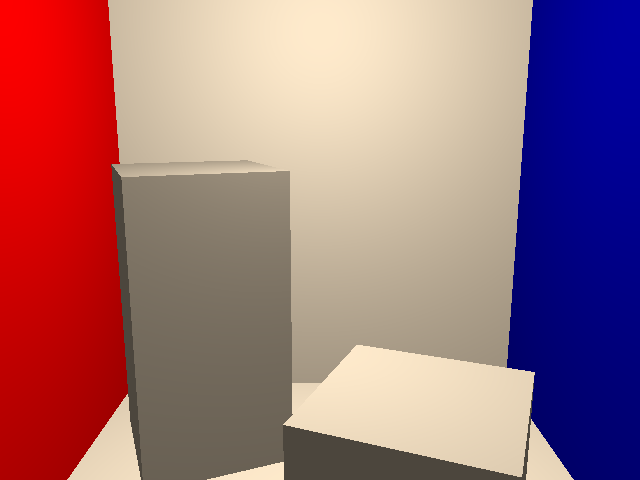
\includegraphics[width=0.3\textwidth]{cornellBox}
  }
  \subfloat[The Reflecting Stanford Dragon.]{
    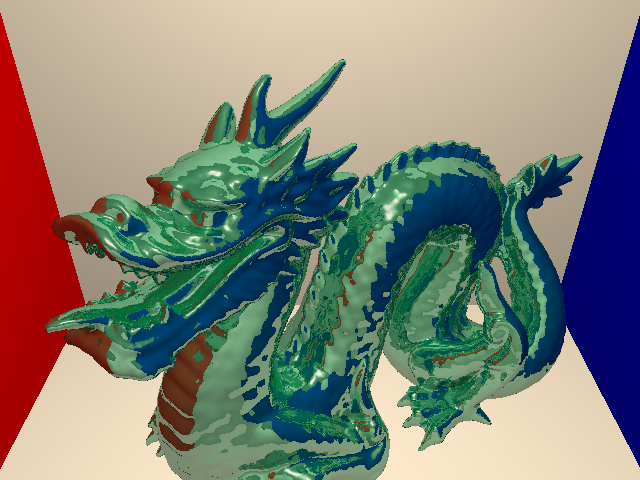
\includegraphics[width=0.3\textwidth]{semiReflectingDragon}
  }
  \subfloat[Sponza.]{
    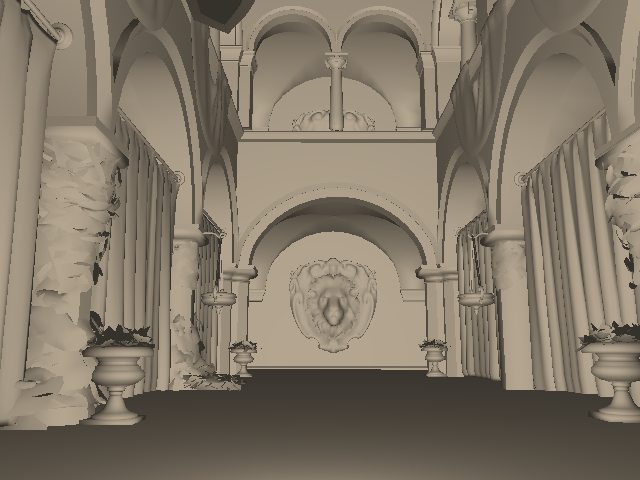
\includegraphics[width=0.3\textwidth]{sponza}
  }
  \caption[Test scenes.]{The 3 test scenes.}
  \label{fig:testScenes}
\end{figure}

% Evaluate ray tracers

% First establish which ray tracer works the best

\begin{tabular} {r | c | c | c || c || c || c ||}
  \multicolumn{4}{c||}{ } & \begin{turn}{45}\begin{tabular}{c}Cornell \\Box\end{tabular}\end{turn} & \begin{turn}{45}\begin{tabular}{c}Reflecting \\Dragon\end{tabular}\end{turn} & \begin{turn}{45}Sponza\end{turn}\\
  \hline
  \multirow{4}{*}{Exhaustive} & \multirow{2}{*}{Moeller} & No packets & N/A & 6 \\
  \cline{3-7}
  & & Packets & N/A & 6 \\
  \cline{2-7}
  & \multirow{2}{*}{Woop} & No packets & N/A & 6 \\
  \cline{3-7}
  & & Packets & N/A & 6 \\
  \hline

  % KD-Restart
  \multirow{8}{*}{KD-Restart} & \multirow{4}{*}{Moeller} & \multirow{2}{*}{No packets} & All Leafs & 6 \\
  \cline{4-7}
  & & & Skip Leafs & 6 \\
  \cline{3-7}
  & & \multirow{2}{*}{Packets} & All Leafs & 6 \\
  \cline{4-7}
  & & & Skip Leafs & 6 \\
  \cline{2-7}
  & \multirow{4}{*}{Woop} & \multirow{2}{*}{No packets} & All Leafs & 6 \\
  \cline{4-7}
  & & & Skip Leafs & 6 \\
  \cline{3-7}
  & & \multirow{2}{*}{Packets} & All Leafs & 6 \\
  \cline{4-7}
  & & & Skip Leafs & 6 \\
  \hline

  % Short-Stack
  \multirow{8}{*}{Short-Stack} & \multirow{4}{*}{Moeller} & \multirow{2}{*}{No packets} & All Leafs & 6 \\
  \cline{4-7}
  & & & Skip Leafs & 6 \\
  \cline{3-7}
  & & \multirow{2}{*}{Packets} & All Leafs & 6 \\
  \cline{4-7}
  & & & Skip Leafs & 6 \\
  \cline{2-7}
  & \multirow{4}{*}{Woop} & \multirow{2}{*}{No packets} & All Leafs & 6 \\
  \cline{4-7}
  & & & Skip Leafs & 6 \\
  \cline{3-7}
  & & \multirow{2}{*}{Packets} & All Leafs & 6 \\
  \cline{4-7}
  & & & Skip Leafs & 6 \\
  \hline
\end{tabular}

%% \begin{tabular}{ r  c  c | c | c | c | c | c | c |}
%% %  & Cornell Box & Reflecting Dragon & Sponza & Fairy Forest \\
%%   &&& \multicolumn{6}{|c|}{Reflecting Dragon - 32bit} \\
%%   \cline{4-9}
%%   &&& \multicolumn{3}{|c|}{None} & \multicolumn{3}{|c|}{Empty Space} \\
%%   \cline{4-9}
%%   &&& Box & Divide & Split & Box & Divide & Split \\
%%   \hline
%%   \multirow{4}{*}{kd-Restart} & \multirow{2}{*}{Moeller} & Leaf Skipping & \\
%%   && All Leafs & \\
%%   \cline{2-8}
%%   & \multirow{2}{*}{Woop} & Leaf Skipping & \\
%%   && All Leafs & \\
%%   \hline
%% \end{tabular}

% Test scenes: Cornell, transparent/reflecting dragon2 and sponza

% Splitting Schemes:

% Profile the time it takes to create the different trees, especially
% the splitting kernels.

% Compare amount of nodes.

% Tree traversal time.

% Warp coherence: balance between traversal steps and intersections =
% high amount of nodes in the leafs ie even less important to spend
% alot of time on that last split.


\chapter{Conclusion}

\chapterquote{The best thing about a boolean is even if you are wrong,
  you are only off by a bit.}{Anonymous}

\chapter{Future Work}\label{chp:future}

\chapterquote{Software is like entropy: It is difficult to grasp,
  weighs nothing, and obeys the Second Law of Thermodynamics; i.e., it
  always increases.}{Norman Augustine}

KD/BVH combination trees: still only carry information for one
dimension, but also provide near and far planes, useful for estimating
the advancement of the ray's $t_{min}$.

Look at stackless raytracers with ropes.

Aila et al.\citebook{Aila2009} has looked at persistent threads to
accelerate raytracing. This could be utilized to accelerate the SAH
calculations of individial nodes.

